
% Cal Poly Thesis
% 
% based on UC Thesis format
%
% modified by Mark Barry 2/07.
%




\documentclass[12pt]{ucthesis}

\newif\ifpdf
\ifx\pdfoutput\undefined
    \pdffalse % we are not running PDFLaTeX
\else
\pdfoutput=1 % we are running PDFLaTeX
\pdftrue \fi

\usepackage{url}
\ifpdf

    \usepackage[pdftex]{graphicx}
    % Update title and author below...
    \usepackage[pdftex,plainpages=false,breaklinks=true,colorlinks=true,urlcolor=blue,citecolor=blue,%
                                       linkcolor=blue,bookmarks=true,bookmarksopen=true,%
                                       bookmarksopenlevel=3,pdfstartview=FitV,
                                       pdfauthor={!!Author goes here!!},
                                       pdftitle={!!Title goes here!!},
                                       pdfkeywords={thesis, masters, cal poly}
                                       ]{hyperref}
    %Options with pdfstartview are FitV, FitB and FitH
    \pdfcompresslevel=1

\else
    \usepackage{graphicx}
\fi

\usepackage{amssymb}
\usepackage{amsmath}
\usepackage[letterpaper]{geometry}
\usepackage[overload]{textcase}
\usepackage{color}

\definecolor{cppCommentGreen}{rgb}{0, 0.4, 0}

\usepackage{listings}
\lstset{
                language=C++,
                basicstyle=\scriptsize\ttfamily,
                keywordstyle=\color{blue}\ttfamily,
                stringstyle=\color{red}\ttfamily,
                commentstyle=\color{cppCommentGreen}\ttfamily,
                morecomment=[l][\color{magenta}]{\#}
                frame=single
                keepspaces=true
                tabsize=4
                numbers=left
                numberstyle=\scriptsize
                numbersep=5pt
}

\bibliographystyle{abbrv}

\setlength{\parindent}{0.25in} \setlength{\parskip}{6pt}

\geometry{verbose,nohead,tmargin=1.25in,bmargin=1in,lmargin=1.5in,rmargin=1.3in}

\setcounter{tocdepth}{2}


% Different font in captions (single-spaced, bold) ------------
\newcommand{\captionfonts}{\small\bf\ssp}

\makeatletter  % Allow the use of @ in command names
\long\def\@makecaption#1#2{%
  \vskip\abovecaptionskip
  \sbox\@tempboxa{{\captionfonts #1: #2}}%
  \ifdim \wd\@tempboxa >\hsize
    {\captionfonts #1: #2\par}
  \else
    \hbox to\hsize{\hfil\box\@tempboxa\hfil}%
  \fi
  \vskip\belowcaptionskip}
\makeatother   % Cancel the effect of \makeatletter
% ---------------------------------------




\begin{document}

% Declarations for Front Matter

% Update fields below!
\title{Real Time Visibility Culling With Hardware Occlusion Queries and Uniform Grids}
\author{Ilya Seletsky}
\degreemonth{June} \degreeyear{2013} \degree{Master of Science}
\defensemonth{June} \defenseyear{2013}
\numberofmembers{3} \chair{Zo\"{e} Wood, Ph.D.} \othermemberA{Foaad Khosmood, Ph.D.} \othermemberB{Aaron Keen, Ph.D.} \field{Computer Science} \campus{San Luis Obispo}
\copyrightyears{seven}	%What does this mean?

\maketitle

\begin{frontmatter}

% Custom made for Cal Poly (by Mark Barry, modified by Andrew Tsui).
\copyrightpage

% Custom made for Cal Poly (by Andrew Tsui).
\committeemembershippage

\begin{abstract}

Culling out non-visible portions of 3D scenes is important for rendering large complex worlds at an interactive frame rate.
Past 3D engines used static prebaked visibility data which was generated using complex algorithms.
Hardware Occlusion Queries are a modern feature that allows engines to determine if objects are invisible on the fly.
This allows for fully dynamic destructible and editable environments as opposed to static prebaked environments of the past.
This paper presents an algorithm that uses Hardware Occlusion Queries to cull fully dynamic scenes in real time.
This algorithm is relatively simple in comparison to other real time occlusion culling techniques, making it possible for the average developer to render large detailed scenes.
It also requires very little work from the artists who design the scenes since no portals, occluders, or other special objects need to be used.

\end{abstract}

%\begin{acknowledgements}

%   Thank you...

%\end{acknowledgements}


\tableofcontents


\listoftables

\listoffigures

\end{frontmatter}

\pagestyle{plain}




\renewcommand{\baselinestretch}{1.66}


% ------------- Main chapters here --------------------





\chapter{Introduction}
\label{intro}

\section{Real Time Graphics}
\label{real-time-graphics}

Real time computer graphics are needed for CAD applications, simulations, video games, and even for just displaying the user interface of an operating system.
Computer graphics can be non-real time, like when doing CGI for a movie.
Each frame can take hours to render, and the result is a very photorealistic image that looks like it's part of the movie itself.
Millions of frames are generated only for each still frame to be visible for a fraction of a second until the next frame to give the illusion of motion.
Real time graphics also display a frame for only a fraction of a second but are rendered on the fly right as the user is controlling the application.
This means the computer can't sit there for hours rendering a frame, it has 33.33 milliseconds if trying to render at 30 frames per second.
Most computer monitors update at 60 Hz so real time graphics typically strive for 60 FPS giving an even smoother experience, and this means the computer now only has 16.66 milliseconds to render a frame.
Maintining a smooth, also known as interactive, framerate is important for ensuring the user has a good experience controlling the application.\cite{Interactive}

\section{Visibility Culling}
\label{visibility-culling}

Modern graphics hardware is becoming better and better at rendering large detailed environments in real time.
Games like Rage, Crysis, Skyrim, Battlefield 3, Just Cause 2, and Grand Theft Auto have maps on an epic scale with drawing distances of several kilometers.
These kinds of environments are achievable by avoiding drawing as much of the world as possible.\cite{heir-occ-map, large-occluders, Vis-Computations-Densely-Occluded, Portal-culling, Cryengine-culling-explained, Portals-mirrors, dpvs, cryengine3, culling-bf, CHC, CHCpp}
This is the job of a visibility culling algorithm.  It's relatively easy to avoid drawing portions of the scene that aren't even in the camera's field of view with view frustum culling.
If a camera is looking at a wall or a mountain in the distance, it's also best to avoid drawing things behind those objects.
With large scenes, it's possible that only about 1\% of it has to be rendered.

The GPU is very good at drawing geometry.
Modern hardware can render many triangles with relative ease.
For example, the dPVS paper has one scene displaying approximately 180,000 triangles at about 68 FPS.\cite{dpvs}
It's perfectly fine for the algorithm to have some false positives when rendering a few objects that are actually not visible.
This would just cause a negligible performance drop that the hardware can just brush off.\cite{large-occluders}
The visual quality starts to suffer if objects go missing that should actually be there, so false negatives on visibility should be avoided.
Most of the visibility culling work happens on the CPU while the GPU does all the rendering.
If the CPU is doing too much work finding which objects the GPU shouldn't render, the performance may be worse than if there is no occlusion culling algorithm in the first place.
A good algorithm must strike the perfect balance where the CPU isn't working too hard but is still saving the GPU a lot of work, giving a considerable performance increase.

\section{Dynamic Environments}
\label{dynamic-environments}

Static environments of the past used prebaking steps to compute things like lighting and visibility.
Nowadays more is possible with fully destructible environments and WYSIWYG level editors built right into the game.
Environments can be made out of modular set pieces and put together like lego blocks.
Figures \ref{fig:hangar-view} and \ref{fig:hangar-peices} show an example.
A wall, column, railing, ladder, or tree may be reused many times in the level, saving artists a lot of work as well as keeping memory down due to loading in one resource and reusing it many times.
This will make the engine work with a mesh soup.

\begin{figure}
\begin{center}
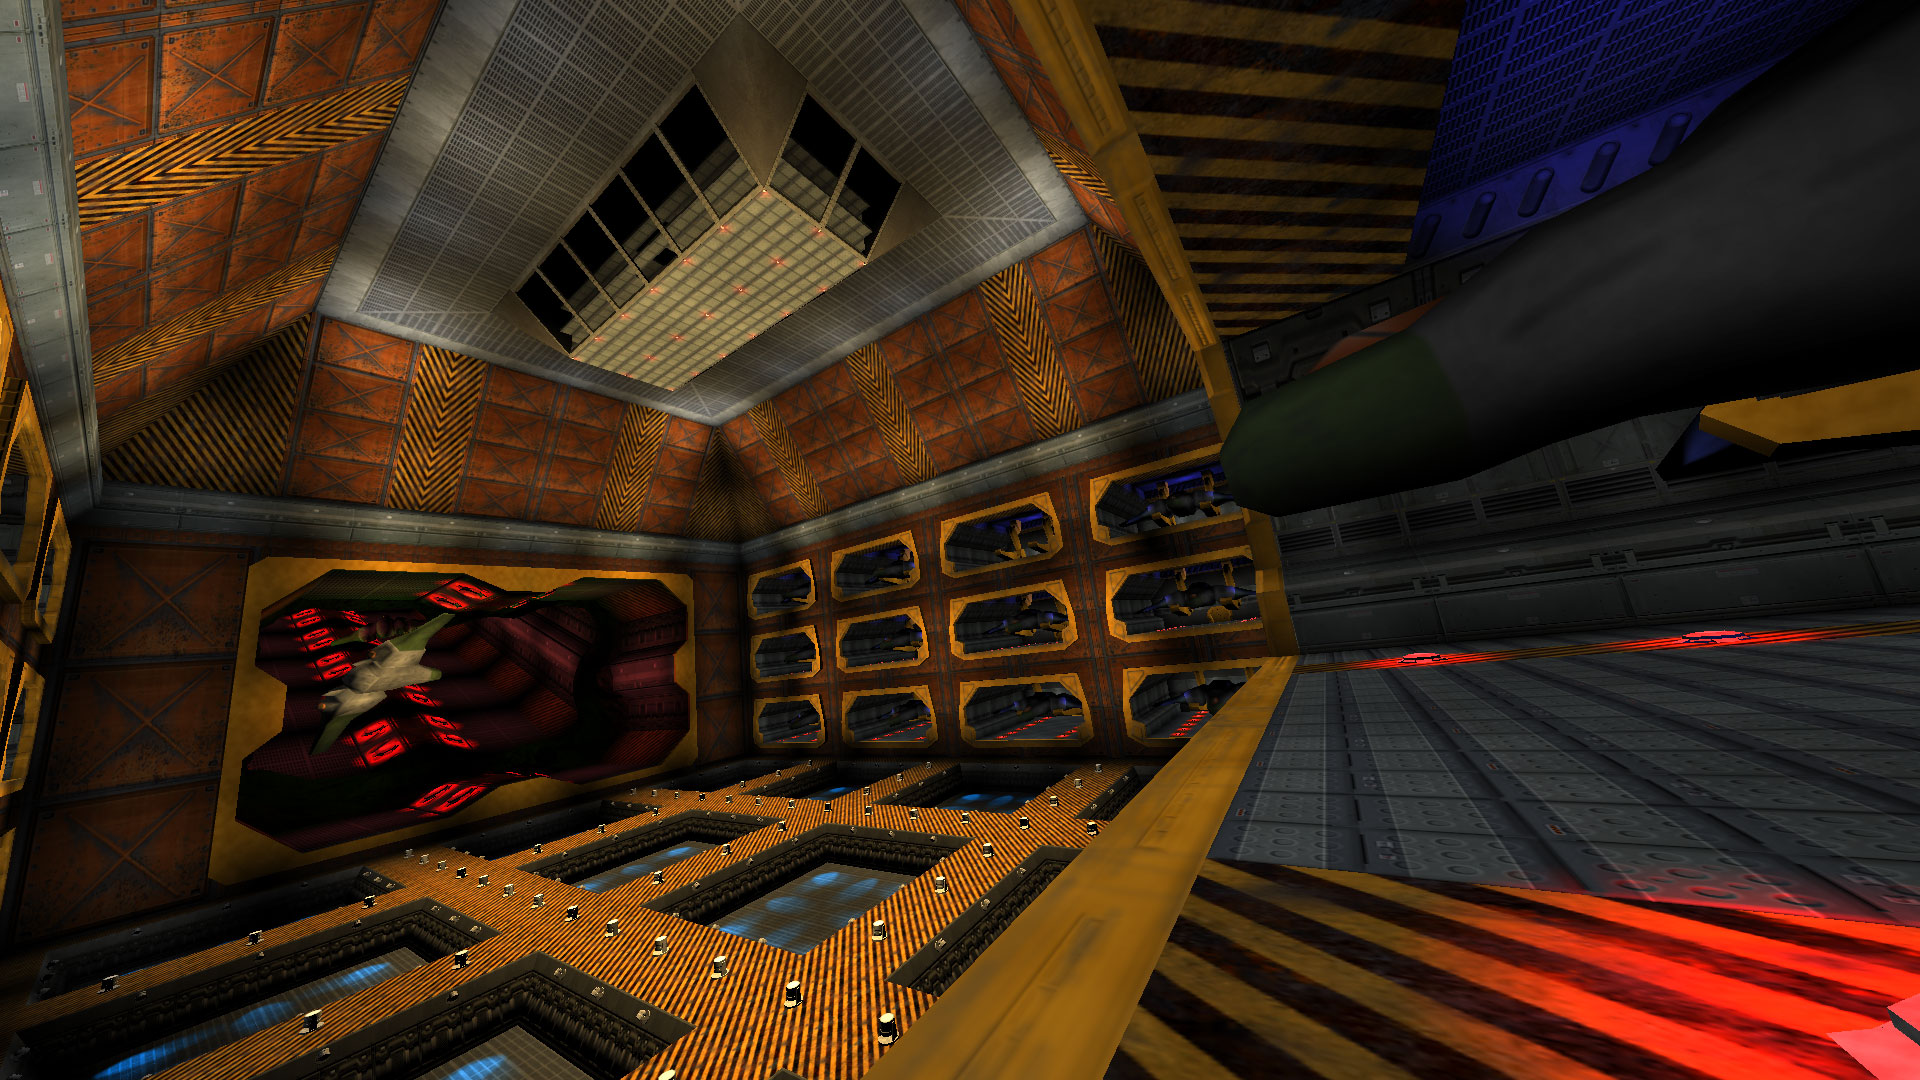
\includegraphics[width=\textwidth]{Images/Hangar.jpg}
\captionfonts
\caption[Hangar]{A view of the Hangar in the environment made for this project.}
\label{fig:hangar-view}
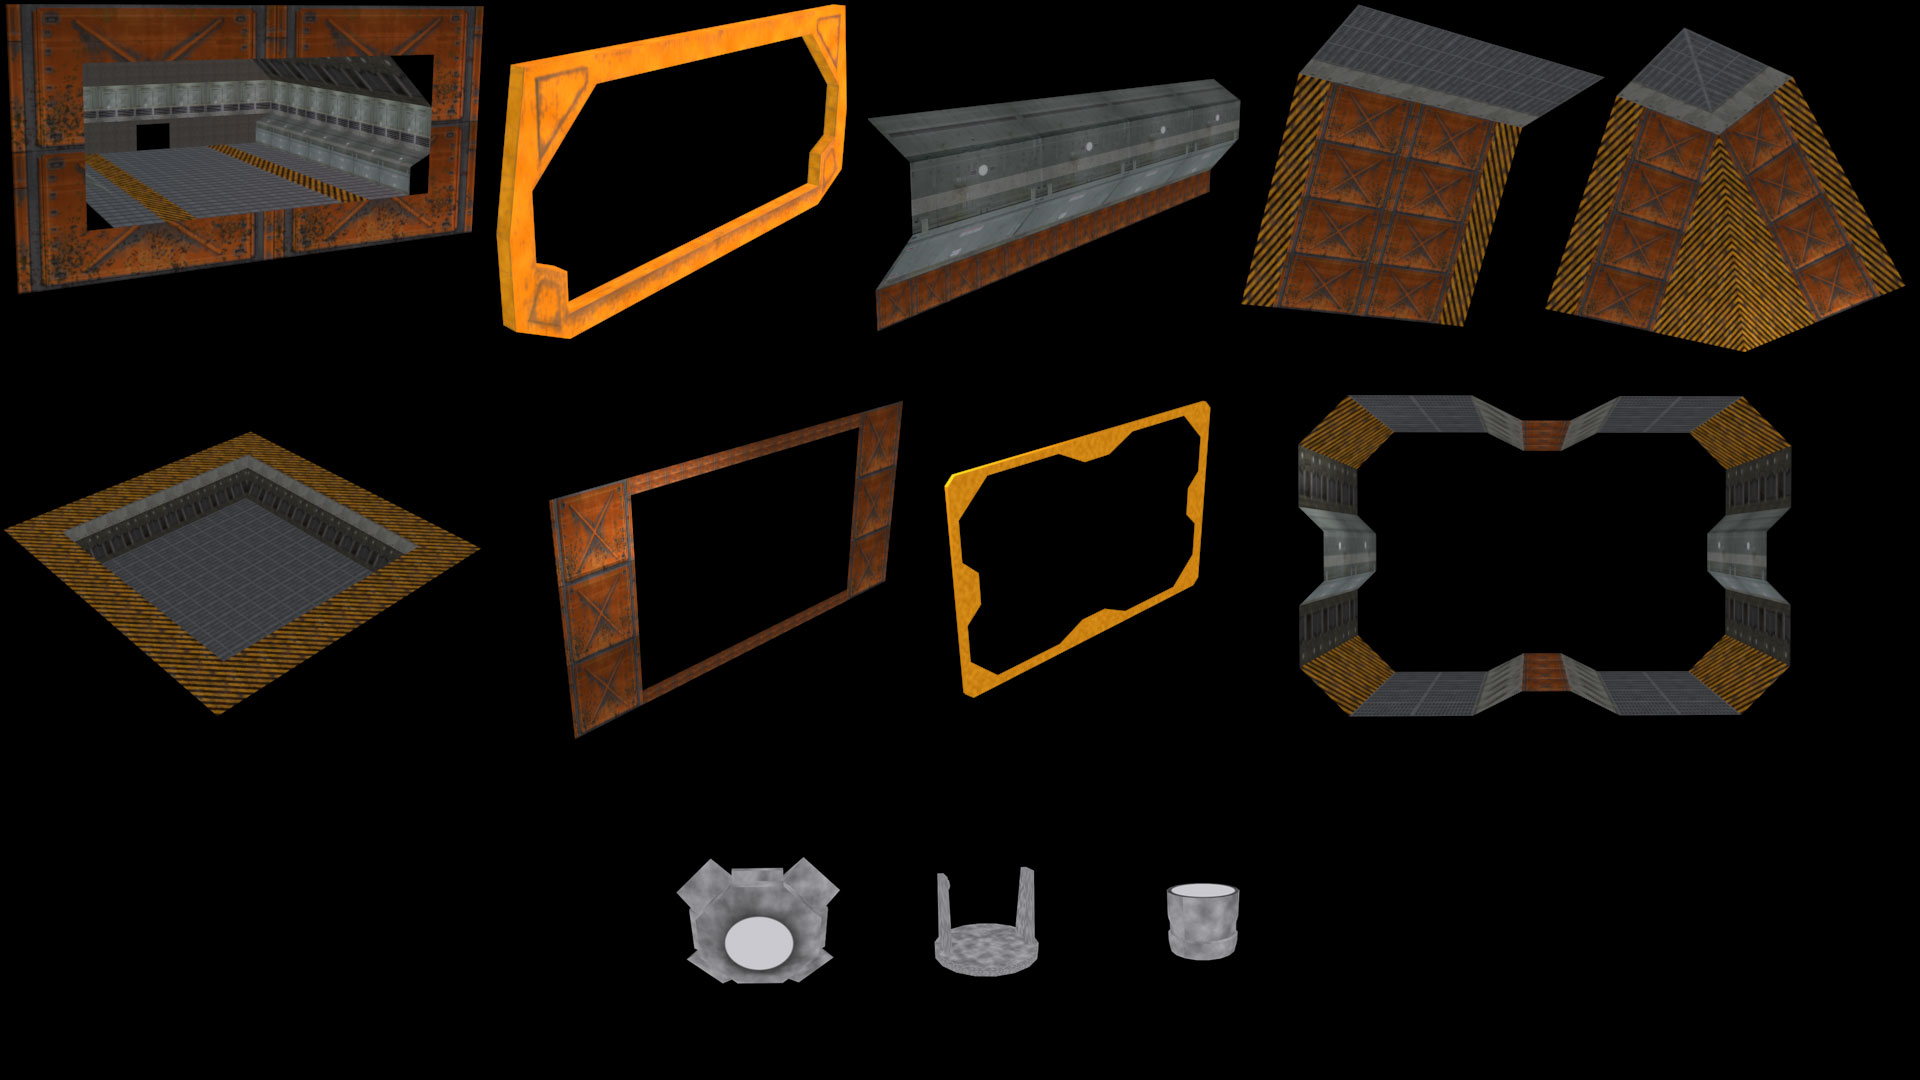
\includegraphics[width=\textwidth]{Images/Peices.jpg}
\captionfonts
\caption[Hangar Modular Pieces]{Some of the modular pieces that make up the hangar.}
\label{fig:hangar-peices}
\end{center}
\end{figure}
While designing levels, the artists would work with these objects by throwing in new ones, moving them around, and deleting them.
The level editor's performance can be greatly increased if it uses a real time visibility culling  algorithm.
In a game with destructible environments, these same objects can now be moved around and destroyed on the fly.
With all of this happening, visibility data needs to update automatically and in real time.
In fact, the level editor can be either built right into the game or just use the same 3D engine that that game uses.
This lets artists see exactly how the environment looks as if they were currently playing the game.

\section{Artist Placed Hint Objects}
\label{artist-placed-hint-objects}

Sometimes an algorithm can't figure out the best way to perform visibility culling in every situation so artists need to place special objects.
This creates a lot of extra work for the artists and can be really tedious.
Artists now need to be educated on the technical inner workings of the engine so they can place the hint objects in the best way.
Even then, artists may still not do it the best way.

Portals are objects that are placed in windows and doorways linking different rooms or zones of an indoor environment.\cite{Vis-Computations-Densely-Occluded, Doom3-source-review, Portal-culling}
They help the engine render objects only visible to the camera through the portal geometry and not through the walls.
They are effective in static environments where the artists know a door or window will always be around.
However if someone takes a rocket launcher and blows up a hole in a wall, there is no artist placed portal there to help the engine.
The engine won't necessarily be smart enough to know how to best place a portal there since any kind of arbitrary destruction can take place.
The zones divided by portals are often static as well and the engine would need to somehow figure out how to create new zones on the fly.
Portals can also be very tedious for the level designers to keep track of as they are constantly iterating on the design of a level.

\begin{figure}
\begin{center}
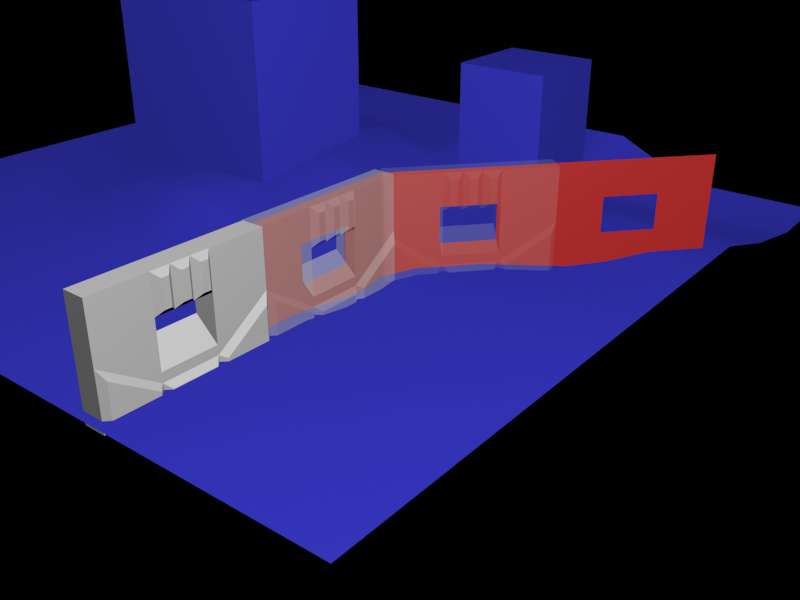
\includegraphics[width=0.75\textwidth]{Images/OccluderGeomFig.jpg}
\captionfonts
\caption[Occluder Geometry]{The detailed wall and its associated low detail occluder geometry shown in red.}
\label{fig:occluder-geometry}
\end{center}
\end{figure}

Occluder geometry is also often used in modern game engines.
Modelers can make a low detail version of a mesh.\cite{culling-bf}
The engine can then do ray intersection tests against all triangles in this mesh to test if some object is behind the geometry.\cite{Cryengine-culling-explained}
Engines that do software occlusion culling render these meshes CPU side rather than rendering the detailed geometry the GPU powered hardware occlusion queries would render.
Making these low resolution meshes that are used specifically for occlusion culling creates extra work for modelers.
If an object is destructible, the low resolution mesh must somehow be deformable along with the high resolution mesh it represents.

\section{Our Contribution}
\label{our-contribution}
This paper presents a simple high performing visibility culling algorithm that any 3D engine can integrate.
It allows rendering of large outdoor worlds that are seamlessly combined with detailed indoor architecture.
It requires hardware that supports occlusion queries, which have been available since about 2003.\cite{GpuGem-Queries}

This algorithm avoids the added complexity of a software rasterizer.
Similar algorithms use software occlusion queries in order to avoid the delay when retrieving hardware occlusion query results.\cite{culling-bf}
This would require software rasterizers to be written that run on the CPU instead of making use of the hardware that performs this task far more efficiently.
The paper also presents a method for combining the use of queries with effective render state sorting.

There is very minimal artist intervention required when designing environments using this algorithm.
The high detail objects that are rendered are also automatically occluding parts of the environment without the need for artists to manually tweak things with portals or special occluding geometry.

A front to back view frustum scene traversal algorithm is presented in order to make the query results optimal.
If the objects in front are drawn before the objects behind, the objects behind can be tested against those already drawn objects.
This reduces false positives in visibility tests.

\chapter{Background}
\label{background}

\section{Z Buffer and Depth Test}
\label{z-buffer-and-depth-test}

The z buffer is allocated along with the buffer to where the image is rendered.
A depth value gets computed for each fragment, which corresponds to a pixel, of a triangle as it gets rasterized by the graphics hardware.
The early z test happens right before the work of the fragment shader where the color of the pixel gets computed and written.\cite{d3d11-pipeline}
The graphics hardware compares the depth value of the fragment about to be written with the value already written.
By default, OpenGL is set to allow a fragment to pass if the new value is less than the current value.\cite{gl-depth-func}
This test is used for solid geometry only, which usually makes up most of the geometry in the scene.
This means solid polygons don't need to be presorted by depth to have the scene look correct.
The depth test is also essential for Hardware Occlusion queries which will be described later.

\section{Other Tests}
\label{other-tests}

There are a few other tests done by the graphics pipeline that can potentially eliminate a fragment.\cite{GpuGem-Occlusion}
The scissor test allows the setting a rectangle on the screen that is rendered to.
Anything outside the scissor rectangle is not rasterized.
The alpha test prevents a fragment from being rendered if the alpha portion of the color is below a certain threshold.
The stencil test uses a buffer similar to the z buffer.\cite{d3d11-pipeline}
Values can be rasterized to the stencil buffer and tested in some way.
If the test passes early on, the fragment can be rasterized if it passes other tests.

\begin{figure}
\begin{center}
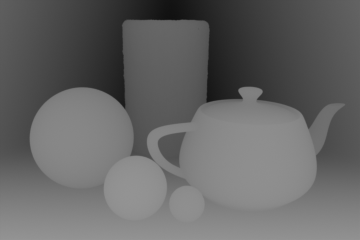
\includegraphics{Images/Z_buffer.png}
\captionfonts
\caption[Z Buffer]{TODO: scale this nicely}
\label{fig:z-buffer}
\end{center}
\end{figure}

\section{Hardware Occlusion Queries}
\label{hardware-occlusion-queries}

The hardware occlusion query is a relatively new feature that is essential to this paper.
The query measures how many fragments have passed for a set of draw calls.
If all fragments have passed all tests of the graphics pipeline described earlier, the query will return a positive result.

\begin{lstlisting}
//creating a query in OpenGL
GLuint query;
glGenQueries(1, &query);

//start the query before a set of draw calls
glBeginQuery(GL_ANY_SAMPLES_PASSED, query);

//some draw calls
glDrawRangeElements(GL_TRIANGLES, ...);

glBegin(GL_QUADS);
    /*some deprecated immediate mode code 
    which you should avoid doing.
    This too works during occlusion queries.
    */
glEnd();

glDrawRangeElements(GL_TRIANGLES, ...);
glDrawRangeElements(GL_TRIANGLES, ...);

//end the query after all those draw calls
glEndQuery();

//getting the result of a query
GLint result;
glGetQueryObjectiv(query, GL_QUERY_RESULT, &result);

//check if query passed
if(result) {
    //do the real rendering
}
\end{lstlisting}

A possible use of a hardware query is to render a simple easy to draw bounding box with color and depth writing disabled.
This means the box will never affect the final image, but it will still go through the full pipeline.
If this box passes all of the pipeline's tests, the real object can be drawn.
However, this is a naive approach that will negatively affect performance.

The problem with hardware occlusion queries is their results may not be ready to read back when expected.\cite{GpuGem-Occlusion, GpuGem-Queries, CHC, CHCpp}
The glGetQueryObject call may cause a CPU stall with the results often being available about 3 to 4 frames later.
The challenge with using hardware occlusion queries is finding a way to effectively use them in later frames to reduce CPU stalls and save the GPU from drawing too many unnecessary objects.

\section{Spatial Data Structures}
\label{spatial-data-structures}

Spatial data structures greatly help reduce the search space by filtering out objects that can't possibly be returned.
A data structure must never falseley filter out values that should be returned but it's always safe to return false positives.

The grid is one of the simplest structures.
Objects have a bounding box, and are binned into cells of the grid that overlap with the bounding box.\cite{culling-bf, applications-spatial, chess}
Querying for objects in the grid simply requires indexing into cells of the grid which intersect with the spatial query.
This is an optimal structure for cases when objects are evenly distributed in the world.
This could be an issue if the scene has hundreds of objects in one cell while the rest of the cells have very sparse amounts of objects.
Querying within the bounds of that cell wouldn't reduce the search space by very much.

A spatial hash is similar to a grid but allows the scene to not be constrained within predefined bounds.
The hash has buckets just like a grid has cells, but multiple cells can hash to one bucket.
For example, if the grid is allocated to hold 5 by 5 cells, grid cell (1, 3) would hash to the same bucket as (6, 3).
A standard grid wouldn't be able to handle cell (6, 3) since that's outside of the grid.

Quad trees are a heirarchical datastructure that handles unevenly distributed objects better.\cite{applications-spatial}
It distributes the objects by progressively dividing each cell into four smaller cells until each cell has a small enough number of objects for the application.
Since it is structured as a tree, many cells get filtered out along the traversal before reaching the leaf cells.
Once a path down a traversal isn't taken, all child nodes in the heirarchy are automatically ignored.
This helps filter out many more potential objects than a grid earlier on in the search.
Octrees are a 3D extension of quadtrees and divide each cell into 8 children rather than 4.
This can be extended to other dimensions beyond that as well, to help with problems mapped to multiple dimensions.\cite{applications-spatial}

Bounding volume heirarchies are another common heirarchical structure.\cite{BVH}
This organizes the scene by having each node be a bounding box that contains the bounding boxes of all of its children.
The leaves in the tree contain the objects themselves.
As the tree is traversed, the bounding box of the query is used to determine what set of children to follow if their bounding box also intersects the query object.
This kind of structure allows any arbitrary scene layout while grids and quadtrees are constrained to hold the scene within predefined bounds.

TODO: BSP and K/D trees

\chapter{Previous Work}
\label{previous-work}

Visibility Culling has been performed with a variety of methods over the last decades.
Many clever tricks have been found that take advantage of certain assumptions about a scene, sometimes limiting what kinds of scenes are possible.
Keeping a scene static while performing a walkthrough of an indoor area is common.
Some software-based occlusion culling solutions have been used as well in order to avoid the CPU stalls of hardware occlusion queries.

One visibility culling algorithm uses mathematical properties of convex polyhedral objects to determine visibility on the fly.\cite{large-occluders}
Coorg and Teller find objects in the scene that serve as large occluders, and avoid testing against smaller objects that wouldn't serve as effective occluders.
Since the environments are made of collections of convex geometry, it's possible to compute separating and supporting planes from pairs of objects and compute whether or not one object is occluding another.
The algorithm was developed at a time when the z buffer may be unavailable or done slowly in software, so this algorithm was able to avoid relying on the z buffer.

Portal culling, which was mentioned earlier, is a very effective technique that many engines can easily implement.
Portals are typically useful in indoor environments and aren't effective in outdoor environments.\cite{Portals-mirrors}
If the environment is subdivided into zones, only geometry in zones that are determined to be visible gets rendered.
The camera's initial view frustum gets computed.
The geometry in the zone the camera is located is then rendered.
If the geometry of a portal is visible to the camera, a new smaller view frustum spawns off that simulates the view through the portal into the adjacent zone.
The scene's zones are traversed this way until no more portals are determined to be visible.

\begin{figure}
\begin{center}
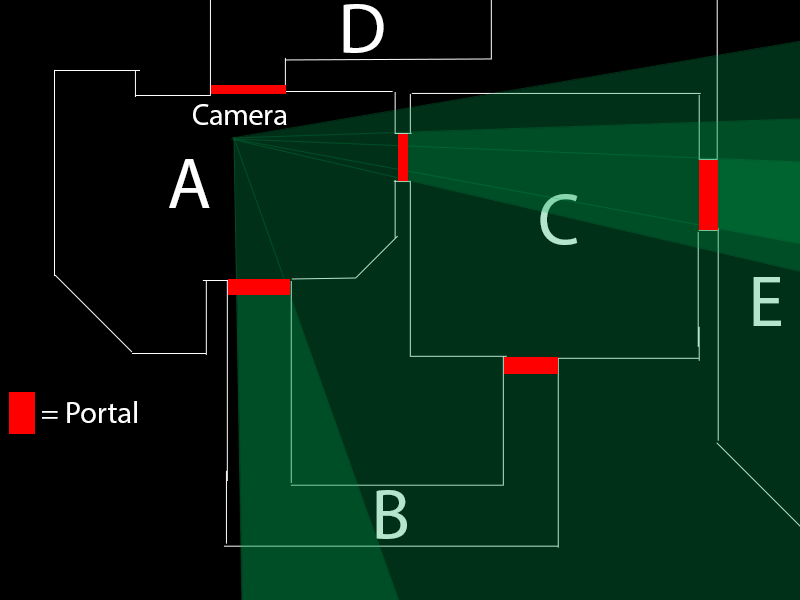
\includegraphics[width=0.75\textwidth]{Images/Portal-Culling.png}
\captionfonts
\caption[Portal Culling]{An example of portal culling at work.  Zones A, B, C, and E are rendered.}
\label{fig:portal-culling}
\end{center}
\end{figure}

Teller finds another way to compute visibility in environments made of convex polyhedral geometry.\cite{Vis-Computations-Densely-Occluded}
This time the scene is preprocessed ahead of time with his algorithm.
The algorithm is applied in id Software's idTech 4 engine used in games like Doom 3 and Quake 4.\cite{Doom3-source-review}
Areas of the environment are subdivided and stored in a BSP tree.
Portals need to be placed by the level designers in crucial areas like doorways and windows to allow the algorithm to compute zones.
The areas determined by the algorithm are joined into zones with a flood filling algorithm.
Solid geometry and artist placed portals determine the bounds of zones.
Without artist placed portals, Doom 3 renders the entire level rather than only visible rooms.
In 1992, this algorithm was said to take hours of CPU time, but was able to store the processed scene in a fraction of the space.
Id software's previous titles, Quake 1 through 3, used to run a similar algorithm offline in a separate utility.
Artists made levels in a separate tool and converted the levels to a format loadable by the game.
Doom 3 can now run this algorithm right before loading a level and the process is built right into the game.
This way the game can ship with the levels in their editable form for people to look at with the built in map editor.

Zang, Manocha, Hudson, and Hoff have developed an algorithm that uses a heirarchy of occlusion maps.\cite{heir-occ-map}
Occlusion maps are similar to the z buffer.
In this algorithm a heirarchy of buffers is created, which are basically the z buffer at different levels of detail.
Occluders are rendered to this buffer.
Occludees then are tested against the right buffer depending on how big they are on the screen by testing and rasterizing a bounding rectangle.
An algorithm similar to this was applied in Ubisoft's Splinter Cell Conviction.\cite{spliter}
They were able to acheive about 20,000 queries every frame on the Xbox 360.

The Frostbite 2 Engine developed by Dice is a great example of modern occlusion culling.\cite{culling-bf}
This engine effectively supports destructible environments in both indoor and outdoor settings as shown in the game Battlefield 3.
It shows off the capabilities of modern high end hardware as well as managing to run on dated hardware with a lower spec profile.
Typically hierarchical data structures such as Octrees, Bounding Volume Hierarchies, or BSP Trees are used for 3D scene management.\cite{CHC, CHCpp, GpuGem-Queries, dpvs}
However, the developers of Battlefield 3 found they were able to push more performance with a uniform grid.
Modern parallel computing architectures handle the linear arrays of a grid much better than the branch heavy traversal of the hierarchical structures.\cite{culling-bf}
The lack of branching creates predictable data access that is cache coherent and allows variaous parallel algorithms to operate more efficiently.
The visibility culling algorithm relies on artist generated low detail large occluder geometry that is rasterized software-side to a low resolution depth buffer.
This requires a software rasterizer capable of rendering arbitrary geometry to be implemented.
Objects such as tanks or soldiers have their bounding rectangle tested against this buffer similarly to how a hardware occlusion query would operate before being queued up for the hardware to render.

CryENGINE 3, used for games like Crysis 2 and Farcry 3, is another modern game engine capable of rendering large indoor and outdoor environments effectively.\cite{cryengine3, Cryengine-culling-explained}
Cryengine uses what is called a coverage buffer but avoids implementing a full arbitrary geometry rasterizer by reading back the z buffer from the hardware and using it in later frames.
As the camera moves around, the coverage buffer needs to be adjusted to correspond more closely to how the current frame looks.
Cryengine reprojects the buffer with the transform of the current camera and then fills in any holes.
After this, like Frostbite 2, objects' bounding rectangles are rasterized and tested against the contents of the coverage buffer.
Cryengine also allows for use of portals and occlusion geometry that they refer to as antiportals to further augment the visibulity culling algorithm.

The dPVS algorithm developed by Aila and Miettenen is another similar algorithm capable of rendering large dynamic environments.\cite{dpvs}
Their system allows for a combination of various occlusion culling algorithms such as portals and queries.
The scene is organized by a K/D tree.
This data structure is normally used best in static environments, but this algorithm is able to effectively recompute the structure on the fly.
They too use a coverage buffer for occlusion queries where the sillhouettes of objects are rasterized.
Queries are then run against this coverage buffer.

The Coherent Heirarchical Culling algorithm uses the same hardware occlusion queries that this paper uses.\cite{CHC, CHCpp}
This algorithm allows a scene managed by a Bounding Volume Heirarchy to effectively use queries.
Temporal coherence is taken advantage of, meaning the results of queries from previous frames are not likely to change.
As the tree of the bounding volume heirarchy is traversed, the visibility results of nodes are used in later frames.
Since this is a heirarchy, entire portions of the scene can be culled out for a number of frames.
They make no mention on whether or not objects noticeably pop in late with this algorithm.

\chapter{Visbility Culling Algorithm}
\label{visibility-culling-algorithm}

\section{Scene Management}
\label{scene-management}

\subsection{Uniform Grid}
\label{uniform-grid}

Typically hierarchical data structures such as Octrees, Bounding Volume Hierarchies, or BSP Trees are used for 3D scene management.\cite{CHC, CHCpp, GpuGem-Queries, dpvs}
A grid, however, is very easy to keep updated with the contents of a fully dynamic scene.
Objects that move around can use their Axis Aligned Bounding Box to determine which cells they need to be tracked in.
A grid's structure doesn't need to be recomputed as the scene changes in real time like the other static structures would.

Modern parallel computing architectures handle the linear arrays of a grid much better than the branch heavy traversal of the hierarchical structures.\cite{culling-bf}
The lack of branching creates predictable data access that is cache coherent.
Modern game engines like Dice's Frostbite 2 use the grid for these reasons.\cite{culling-bf}
The performance of Battlefield 3 is a good example of the simple uniform grid's effectiveness in managing large dynamic environments.

\subsection{Objects at Cell Boundaries}
\label{objects-at-cell-boundaries}
When doing spatial queries against a grid, some group of cells gets traversed and all objects in those cells get returned in the query.
If an object occupies multiple cells it can potentially get added multiple times as a query result.
Keeping track of a 64 bit unsigned query id counter can prevent this.
The main scene can store a query counter, and increment it every time a query occurs.
The objects returned by the query can keep a query counter within them as well.
If the object's counter is less than the scene's counter, then the object hasn't been added to the query results yet.
As the object is added, its counter is set to the scene's counter and any other cells that contain the object won't needlessly duplicate the object in the query.

In a multithreaded engine, when many queries can occur in parallel, a lockless set of query ids per object can work.
If a query id is already in the object's query set, the object can be ignored.
After the query results are done, the query id can be removed from the set, keeping the set from growing.
Lockless sets that are part of Intel Thread Building Blocks don't allow safe lockless removal, so it may be best to clear these sets at some synchronization point such as the end of a frame to prevent them from growing too large.\cite{tbb}

\section{Grid View Frustum Culling}
\label{grid-view-frustum-culling}

\subsection{Overview}
\label{Overview}
The view frustum culling occurs on the grid cells only, rather than on each individual object in the scene.
This allows all objects grouped in a cell to be culled out at once rather than making the CPU check every object individually.
If a cell is right at the border of the view frustum and a few objects inside the cell aren't in the frustum, it's not a problem to have the GPU needlessly render them.
The work done by the CPU checking all objects in a cell will cause a higher performance drop than having the GPU draw a few wasted objects.
This algorithm allows for large scenes with fine enough grids that there will usually be very few wasted objects compared to the immense number of objects that do get rendered.

The cells in the grid should be traversed front to back relative to the view.
This way objects closer to the camera get rendered to the z buffer before objects in the back do.
Cells farther from the camera get tested against the objects in front that are potentially occluding them since they are in the z buffer.

A true front to back traversal of a grid is very difficult to do well.
One attempt involved traversing out with rays from the center and stopping the traversal when reaching an occluded cell or the far plane.
This method never made it past the paper planning stage.
There was a lot of difficulty in figuring out the best way to align the rays so that duplicate cell traversals were minimized and absolutely no cells were ever missed.

Another method for grid traversal uses the chessboard metric. %(http://www.dca.fee.unicamp.br/projects/mtk/batageloM/batagelo-wu-2002-cgf.pdf)
Each slice of the frustum is determined by traversing cells that are a certain grid distance away from the origin.
The distance is increased by 1 each slice.
The view vector itself is rasterized as a line in 3D using the DDA algorithm.
The cells that make up the points of the rasterized line are used as origin points from where traversal should fan out for that slice.
This algorithm made it difficult to avoid traversing cells completely outside of the view frustum.
When the view is at an angle, there is a huge space past the far plane that ends up being needlessly traversed.
Modifying the algorithm to avoid this, especially extended to 3D, was too messy.

The final idea involves taking axis aligned slices of the grid perpendicular to the highest magnitude component of the view vector.
It's a simple algorithm compared to the previously tried solutions and can be based on existing convex polygon rasterization algorithms but extended to 3D.
This isn't a true front to back traversal but it provides the needed results.
In the figure below, cell 8 is traversed after cell 7, but cell 8 is closer in distance.
However, cell 7 will never occupy space in front of cell 8, so any objects in cell 7 will never be drawn in front of cell 8.
Cell 8 will be occluded by objects in cell 3 and 0, while cell 7 will most likely by occluded by objects in cells 6, 5, 2, 1, and 0.
As long as a cell is traversed after the cells that could potentially occlude it, the query results will be optimal and not create false positives.
This gives a true occlusion order traversal but not a true depth order traversal.
This same traversal order is also perfect for roughly depth sorting alpha blended objects that will need to be rendered later.
A shorter sub sort per cell rather than sorting over the entire list of objects to render can give the correct rendering order for transparent objects.
This depth sorting can even be parallelized by using a separate thread per cell, however this hasn't been tried yet in the current renderer.

\subsection{Handling Wide Fields of View}
\label{handling-wide-fields-of-view}
In practice, view frustums are very wide.
A camera using a 90 degree vertical field of view on a 16:9 wide screen monitor will do this.
Wide frustums cause cells that should have been occluded to be traversed before the cells that occlude them.
In this case cell 0 is most likely occluded by cells 3, 4, and 5.
Even if the camera is staring straight at a wall, cells 0, 1, and 2 will falsely pass the occlusion queries because the wall in cell 3 hasn't been rendered to the z buffer yet.

Splitting the frustum into pieces solves this.
The splitting point is centered around the cell where the eye is located.
This creates new convex volumes out of the split view frustum.
In 3D, the frustum is split into 8 pieces by the x, y, and z planes.
A convex polygon plane clipping algorithm will do the trick.
The volumes are now traversed in a fan out order around the center cell.
In the figure below, first the central volume is traversed, and then cells 22, 23, and 24 are traversed afterwards.
This keeps the correct occluder order and avoids false positives.

\subsection{The Rasterizing Algorithm}
\label{the-rasterizing-algorithm}
TODO: should I go into the 3D rasterizing here?  Should I put it in the appendix?

\section{Rendering}
\label{rendering}

\subsection{Render State Sorting}
\label {render-state-sorting}
Other rendering algorithms that make use of hardware occlusion queries usually benefit from having all objects sorted front to back.
This way a tree in front of a dog can potentially occlude the dog.
Then a tree farther in the distance may be occluded by a garbage can.
This would require the objects to be drawn in the order, Tree A, Dog, Garbage Can, Tree B.
Rendering performance would suffer since these objects aren't sorted in an optimal render state order, but in occlusion order.
When rendering a large number of objects, they should be sorted in a way that causes the least amount of change in the render state.
It would be better to render Tree A, Tree B, then switch to the shader and textures that render the dog, then do the same for the garbage can.
The algorithm in this paper avoids this problem and allows objects to be queued up and then sorted by their render state.

The deferred shading renderer used for this project sorts objects first by shader, then textures, then by the instance of mesh.
This is done in order of which changes cause the worst performance hit for the GPU.
It should also be possible to quickly depth sort the meshes being rendered to avoid some overdraw but the objects are already sorted well enough when the view frustum is rasterized front to back.
True depth sort is only needed for alpha blended objects.

\subsection {The Visibility Culling / Depth Pass}
\label{the-visibility-culling-depth-pass}
The first phase involves performing a depth pre pass while performing the occlusion queries.
The depth pre pass renders solid objects to the z buffer with color writing disabled so the complex pixel shaders of the later stages aren't run.
This is used for the occlusion queries during this stage as well as for preventing pixel shader overdraw later.
For each unoccluded cell that is traversed during this phase, its objects are rendered to the z buffer as well as being added to the main render queue.

First, the query results from last frame are gathered so they can be used this frame to know whether a cell was found visible or not.
Since the cell query results are used next frame, objects may pop in a frame late.
This is unnoticeable at high frame rates due to how little time this takes, and is a common sacrifice other engines make when using occlusion queries.
This is the part of the algorithm that takes up about 25\% CPU time.
Query results may take upto four frames to be ready in some cases, so even using the results next frame rather than the current frame causes a CPU stall.
The frame rate still remains high, sometimes reaching 300 FPS if running only queries but not rendering anything.
The call to retrieve the query result blocks the CPU until the result is available, but it is possible to first check if the result is available before making the blocking call.
This is avoided to keep the algorithm simpler and avoid rendering frames where the object isn't visible yet.
This stall can be inconsequential if a separate thread retrieves the query results while the engine is left to run Physics, AI, sound, and other subsystems.

The cells keep track of their last visible frame by storing a 64 bit unsigned frame counter.
A 64 bit unsigned integer can store more atoms than there are in the universe.
Even if the renderer is running at 500 FPS, it will take 15,768,000,000 years for this counter to roll over.
The scene itself keeps track of the current frame counter in its own 64 bit unsigned integer.
When a cell query is retrieved, it writes the current frame counter of the scene as the last visible frame.
This way it's unnecessary to to iterate over all cells every frame to reset their visibility status.

%TODO: source code
%isCellVisibleLastFrame()
%	return cell.lastVisibleFrame == scene.currentFrame - 1;

In order to prevent too much work during the depth pre pass, the artists can specify how the object should be rendered during this phase.
This is one of the only settings artists need to tweak in the environment to push a little extra performance.
The three settings for an object are to always render, sometimes render, and to never render.
An object can be marked as an essential occluder that must always be rendered if its cell is visible.
This is for objects like walls, terrain, or any other objects that keep the world water-tight.
These are objects that must populate the z buffer in order for cells behind to be properly occluded.
The second setting of "sometimes" is reserved for fairly large detail adding objects that would be in the middle of rooms, such as crates, columns, or trees.
The deferred renderer in the game Space Marine limits the depth pre pass to only 75 objects in order to prevent too much work during this phase. %(http://www.slideshare.net/blindrenderer/rendering-tech-of-space-marinekgc-2011)  
This engine only adds objects marked to render sometimes if there aren't already 75 objects rendered in the depth pass.
Since the scene is traversed front to back, the objects close to the camera and likely to contribute to occlusion usually make it while the further away objects are avoided.
The third setting of "never" is for the tiny objects that add detail.
In a fully detailed environment it's likely that there will be very many of these objects.
They are likely to not contribute much to the occlusion and rendering them during this phase can be a waste.
Here the walls, ceiling, and floors are marked to always render.
The fighter jets inside the hangars are marked to sometimes render.
The lamps on the floor and clamps holding the jets in place are marked to never render. (Probably get a screenshot where the fighter jets are easier to make out)
In this outdoor area, The building, underground tunnel walls, and the terrain are set to always render.
The teapots and jets are set to sometimes render.
The red lamps on the building are set to never render.

The following pseudocode shows the algorithm.


The Rendering
Now all objects from cells marked as visible in the previous frame are gathered up and ready to be rendered in color.  They should be sorted by render state as mentioned earlier.  A deferred shading renderer is used for this project, but any kind of renderer can be used.  In this case, solid objects are all queued up in one render state list.  This is a great opportunity to use the batching API available on modern graphics cards to reduce draw calls and render all objects of one type in 1 call.  The depth write and depth test should still be enabled at this time since not all objects were added to the z buffer during the depth pre pass.  The depth test function should be set to less than or equal.  All lights to be rendered during the lighting pass are queued up in another list.  Transparent objects can be queued up in another list in the occlusion order mentioned earlier and rendered using forward rendering.  The same grid that stores objects in the scene can be queried for which lights affect objects to be rendered during forward rendering.
Spreading Queries
Tight detailed indoor environments benefit from the scene using a finer grid.  The hallway in fig 1337 is built around the hangar bay in pictured in fig 6969.  If the grid is too sparse, large chunks of the hangar get rendered that should be occluded by the walls of the hallway because the cells are too big and contain too many objects. 
When inside the hallway, the frame rate is about 60 FPS with a fine grid, and can drop down to 25 FPS with a more sparse grid.  However, having too fine a grid can also be bad for performance overall.  The frustum rasterization algorithm has no problem with traversing extreme amounts of cells, but the querying and rendering of individual cells is the bottleneck.  Depending on the camera position and viewing angle, the number of traversed cells in a fine grid can range from about 500 to 60,000.  There isn?t a good way to batch all of the cubes that get rendered for the cell queries into a single draw call.  The queries happen in between rendering a group of objects to the depth buffer and there seems to be no way to have a query for each individual object in a batch at the moment.  In the worst case, that many draw calls being made causes severe performance drops down to about 4 FPS.

One solution is to try to group far away cells into one query.  It may be possible to modify the frustum rasterizing algorithm to support this in the future.  The grid could be rasterized more like a hierarchical octree.  Any far way grouped cells that are visible can then be subdivided into finer cells in later frames to filter out the portions of the scene that aren't visible.  This would take considerable effort due to the way the rasterizing algorithm is currently built to traverse row by row in the grid.
A simpler solution is to limit the number of queries per frame.  A limit of about 3000 to 4000 produces good results.  Query results now need to last multiple frames.  The algorithm is becoming similar to the Coherent Hierarchical Culling algorithm, in that results of queries are likely to not change too much between frames that are close by in time.  The current algorithm allows successful visibility queries to last for about 30 frames and failed invisible cell queries to last about 2 frames.  A lower number for invisible cells is needed to avoid waiting too long to let previously invisible cells to have their objects pop in noticeably while moving through the scene.  Now if a query result is still valid, the cell doesn't need to be re-queried and cells that haven't been queried in previous frames have a chance.  This can at cause slightly more noticeable pop in of objects while moving since some cells get queried a few frames later at the cost of keeping the frame rate higher.  The frame rate being high reduces the real time it takes for an object to pop in, making it less noticeable anyway, so this tends to be a good tradeoff.
Moving sideways can make far away objects seen through the door sometimes appear to pop in visibly if someone is really paying attention.  A high frame rate and an action packed game help ensure this artifact is hard to notice.
Query Starvation
When a large amount of cells needs to be queried, some cells never have a chance and patches of the world go missing.  Cells early in the frustum traversal whose query results have expired eat up the queries that farther away cells need to become visible.  If 40,000 cells need to be queried, and nonvisible cell results last only 2 frames, those same nonvisible cells will keep executing queries. 
Extending the duration of query results when the query cap is hit, as well as offsetting the duration by a random amount, helps avoid the problem of query starvation.  It?s possible to keep track of how many frames in a row have hit the query cap and base the duration extension on this amount.  After a few frames, all cells that should be visible have had a chance to be queried and the scene looks correct.  The popping artifacts stay relatively unnoticeable.

The following pseudocode shows how the current implementation takes into account the number of frames in a row the query cap was hit.  The invisibilityDurationGrowth variable should be smaller than the visibilityDurationGrowth variable to keep the previously described popping artifacts at a minimum while moving.
for each query from last frame
	get query result
	if any samples passed
		mark cell as visible for frameCounter + (visibilityDuration + visibilityDurationGrowth * numFramesOverflowed) + rand(0, numFramesOverflowed * 2);
	else
		mark cell as invisible for frameCounter + (invisibilityDuration + invisibilityDurationGrowth * numFramesOverflowed) + rand(0, numFramesOverflowed * 2);
++frameCounter

Sometimes a few random objects can start blinking every couple frames because a visibility query has expired.  This ends up being noticeable even at high frame rates.  This happens when the query cap has been reached so the visible cell is now invisible until next frame when it can be queried.  This is easily avoided by ignoring the visibility cap for visible cells that need to be re-queried.  This happens rarely enough that only about 2 to 30 cells may sometimes need to violate the cap and there is no negative impact on performance.

The following pseudocode shows modifications to the previous algorithm.
TODO: make the pseudo code better


\chapter{Results}
\label{results}

Here is the results section.

LaTeX is a document markup language and document preparation system for the TeX typesetting program.

It is widely used by mathematicians, scientists, philosophers, engineers, and scholars in academia and the commercial world, and by others as a primary or intermediate format (e.g. translating DocBook and other XML-based formats to PDF) because of the quality of typesetting achievable by TeX. It offers programmable desktop publishing features and extensive facilities for automating most aspects of typesetting and desktop publishing, including numbering and cross-referencing, tables and figures, page layout and bibliographies.

LaTeX is intended to provide a high-level language to access the power of TeX. LaTeX essentially comprises a collection of TeX macros, and a program to process LaTeX documents. Since TeX's formatting commands are very low-level, it is usually much simpler for end-users to use LaTeX.

LaTeX was originally written in 1984 by Leslie Lamport at SRI International and has become the dominant method for using TeX�few people write in plain TeX anymore.

LaTeX is based on the idea that authors should be able to focus on the meaning of what they are writing, without being distracted by the visual presentation of the information. In preparing a LaTeX document, the author specifies the logical structure using familiar concepts such as chapter, section, table, figure, etc., and lets the LaTeX system worry about the presentation of these structures. It therefore encourages the separation of layout from content, while still allowing manual typesetting adjustments where needed. This is similar to the mechanism by which many word processors allow styles to be defined globally for an entire document, or the CSS mechanism used by HTML.

LaTeX can be arbitrarily extended by using the underlying macro language to develop custom formats. Such macros are often collected into packages which are available to address special formatting issues such as complicated mathematical content or graphics. In addition, there are numerous commercial implementations of the entire TeX system, including LaTeX, to which vendors may add extra features like additional typefaces and telephone support. LyX is a free visual document processor that uses LaTeX for a back-end. TeXmacs is a free, WYSIWYG editor with similar functionalities as LaTeX, but a different typesetting engine.

A number of popular commercial desktop publishing systems use modified versions of the original TeX typesetting engine. The recent rise in popularity of XML systems and the demand for large-scale batch production of publication-quality typesetting from such sources has seen a steady increase in the use of LaTeX.


\begin{table}
\begin{center}

\begin{tabular}{|c|c|c|c|c|c|c|}
\hline 
&
\multicolumn{2}{c|}{Some Data}&
&
\multicolumn{2}{c|}{Some More Data}&
\tabularnewline
\hline
\hline 
&  Hi-Res&  Lo-Res&  Reduction&  Hi-Res&  Lo-Res&  Speedup
\tabularnewline
\hline 
Row Data A &  225,467&  43,850&  80.6\%&  360&  90&  4.0
\tabularnewline
\hline 
Row Data B &  225,467&  16,388&  92.7\%&  360&  26&  13.8
\tabularnewline
\hline 
\end{tabular}


\captionfonts
\caption[Performance data]{Here is some performance data for the system.}
\label{table:performance}
\end{center}
\end{table}


LaTeX is a document markup language and document preparation system for the TeX typesetting program.

It is widely used by mathematicians, scientists, philosophers, engineers, and scholars in academia and the commercial world, and by others as a primary or intermediate format (e.g. translating DocBook and other XML-based formats to PDF) because of the quality of typesetting achievable by TeX. It offers programmable desktop publishing features and extensive facilities for automating most aspects of typesetting and desktop publishing, including numbering and cross-referencing, tables and figures, page layout and bibliographies.

LaTeX is intended to provide a high-level language to access the power of TeX. LaTeX essentially comprises a collection of TeX macros, and a program to process LaTeX documents. Since TeX's formatting commands are very low-level, it is usually much simpler for end-users to use LaTeX.

LaTeX was originally written in 1984 by Leslie Lamport at SRI International and has become the dominant method for using TeX�few people write in plain TeX anymore.

LaTeX is based on the idea that authors should be able to focus on the meaning of what they are writing, without being distracted by the visual presentation of the information. In preparing a LaTeX document, the author specifies the logical structure using familiar concepts such as chapter, section, table, figure, etc., and lets the LaTeX system worry about the presentation of these structures. It therefore encourages the separation of layout from content, while still allowing manual typesetting adjustments where needed. This is similar to the mechanism by which many word processors allow styles to be defined globally for an entire document, or the CSS mechanism used by HTML.

LaTeX can be arbitrarily extended by using the underlying macro language to develop custom formats. Such macros are often collected into packages which are available to address special formatting issues such as complicated mathematical content or graphics. In addition, there are numerous commercial implementations of the entire TeX system, including LaTeX, to which vendors may add extra features like additional typefaces and telephone support. LyX is a free visual document processor that uses LaTeX for a back-end. TeXmacs is a free, WYSIWYG editor with similar functionalities as LaTeX, but a different typesetting engine.

A number of popular commercial desktop publishing systems use modified versions of the original TeX typesetting engine. The recent rise in popularity of XML systems and the demand for large-scale batch production of publication-quality typesetting from such sources has seen a steady increase in the use of LaTeX.


% ------------- End main chapters ----------------------

\clearpage
\bibliography{bibliography}
\bibliographystyle{plain}
%\addcontentsline{toc}{chapter}{Bibliography}

\end{document}